\documentclass[main.tex]{subfiles} % Subfile-Class


% ============================================================================== %
%                            Subfile document                                    %
% ============================================================================== %

\begin{document}

% Template

\subsubsection{Antriebe und Dimensionierung}

Dieser Abschnitt beschäftigt sich mit der Auswahl eines passenden Antriebs für
den Pfadfinder. Die Evaluation der Antriebe, siehe Anhang XXXXXXXXXX, hat
ergeben, dass ein Schrittmotor der Firma DFRobot, siehe
Abbildung~\ref{Schrittmotor_FIT0278}, eingesetzt wird. Dieser ist in der Lage,
mit 1.7A den Pfadfinder auf bis zu $2\frac{m}{s}$ zu beschleunigen.

\begin{figure}[H]
    \centering
    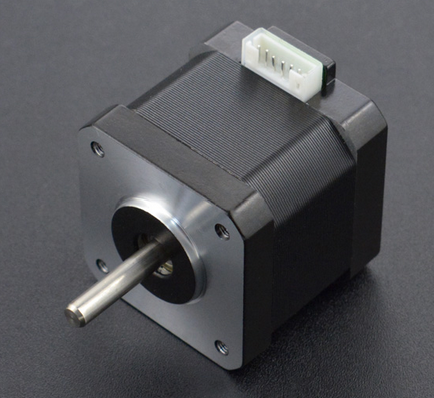
\includegraphics[width = 0.25 \linewidth]{fig_Antriebe_und_Dimensionierung/DFRobot_Stepper_FIT0278.png}
    \caption{Schrittmotor}~\label{Schrittmotor_FIT0278}
\end{figure}

\begin{figure}[H]
    \centering
    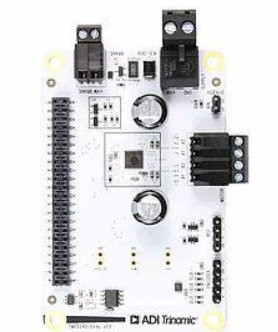
\includegraphics[width = 0.25 \linewidth]{fig_Antriebe_und_Dimensionierung/TMC_5240_EVAL.png}
    \caption{Evaluationboard TMC5240}~\label{Schrittmotorentreiber_EVAL}
\end{figure}

Angesteuert werden diese Motoren über einen Vollintegrierten
Schrittmotorentreiber der Firma ADI-Trinamic. Um weniger Entwicklungsaufwand zu
haben, wird auf 2 Evaluation-Boards des Treiber-IC's \textit{TMC-5240}
zurückgegriffen, gezeigt in Abbildung~\ref{Schrittmotorentreiber_EVAL}. Eines
der Teammitglieder hat bereits Erfahrungen mit diesem speziellen Treiber und
kann auf entsprechende Treiber aus seinem beruflichen Umfeld zurückgreifen.

Die Abbildung~\ref{Ansteuerungstopologie_Schrittmotorentreiber} zeigt
schematisch, wie diese Treiber angesteuert werden.

\begin{figure}[H]
    \centering
    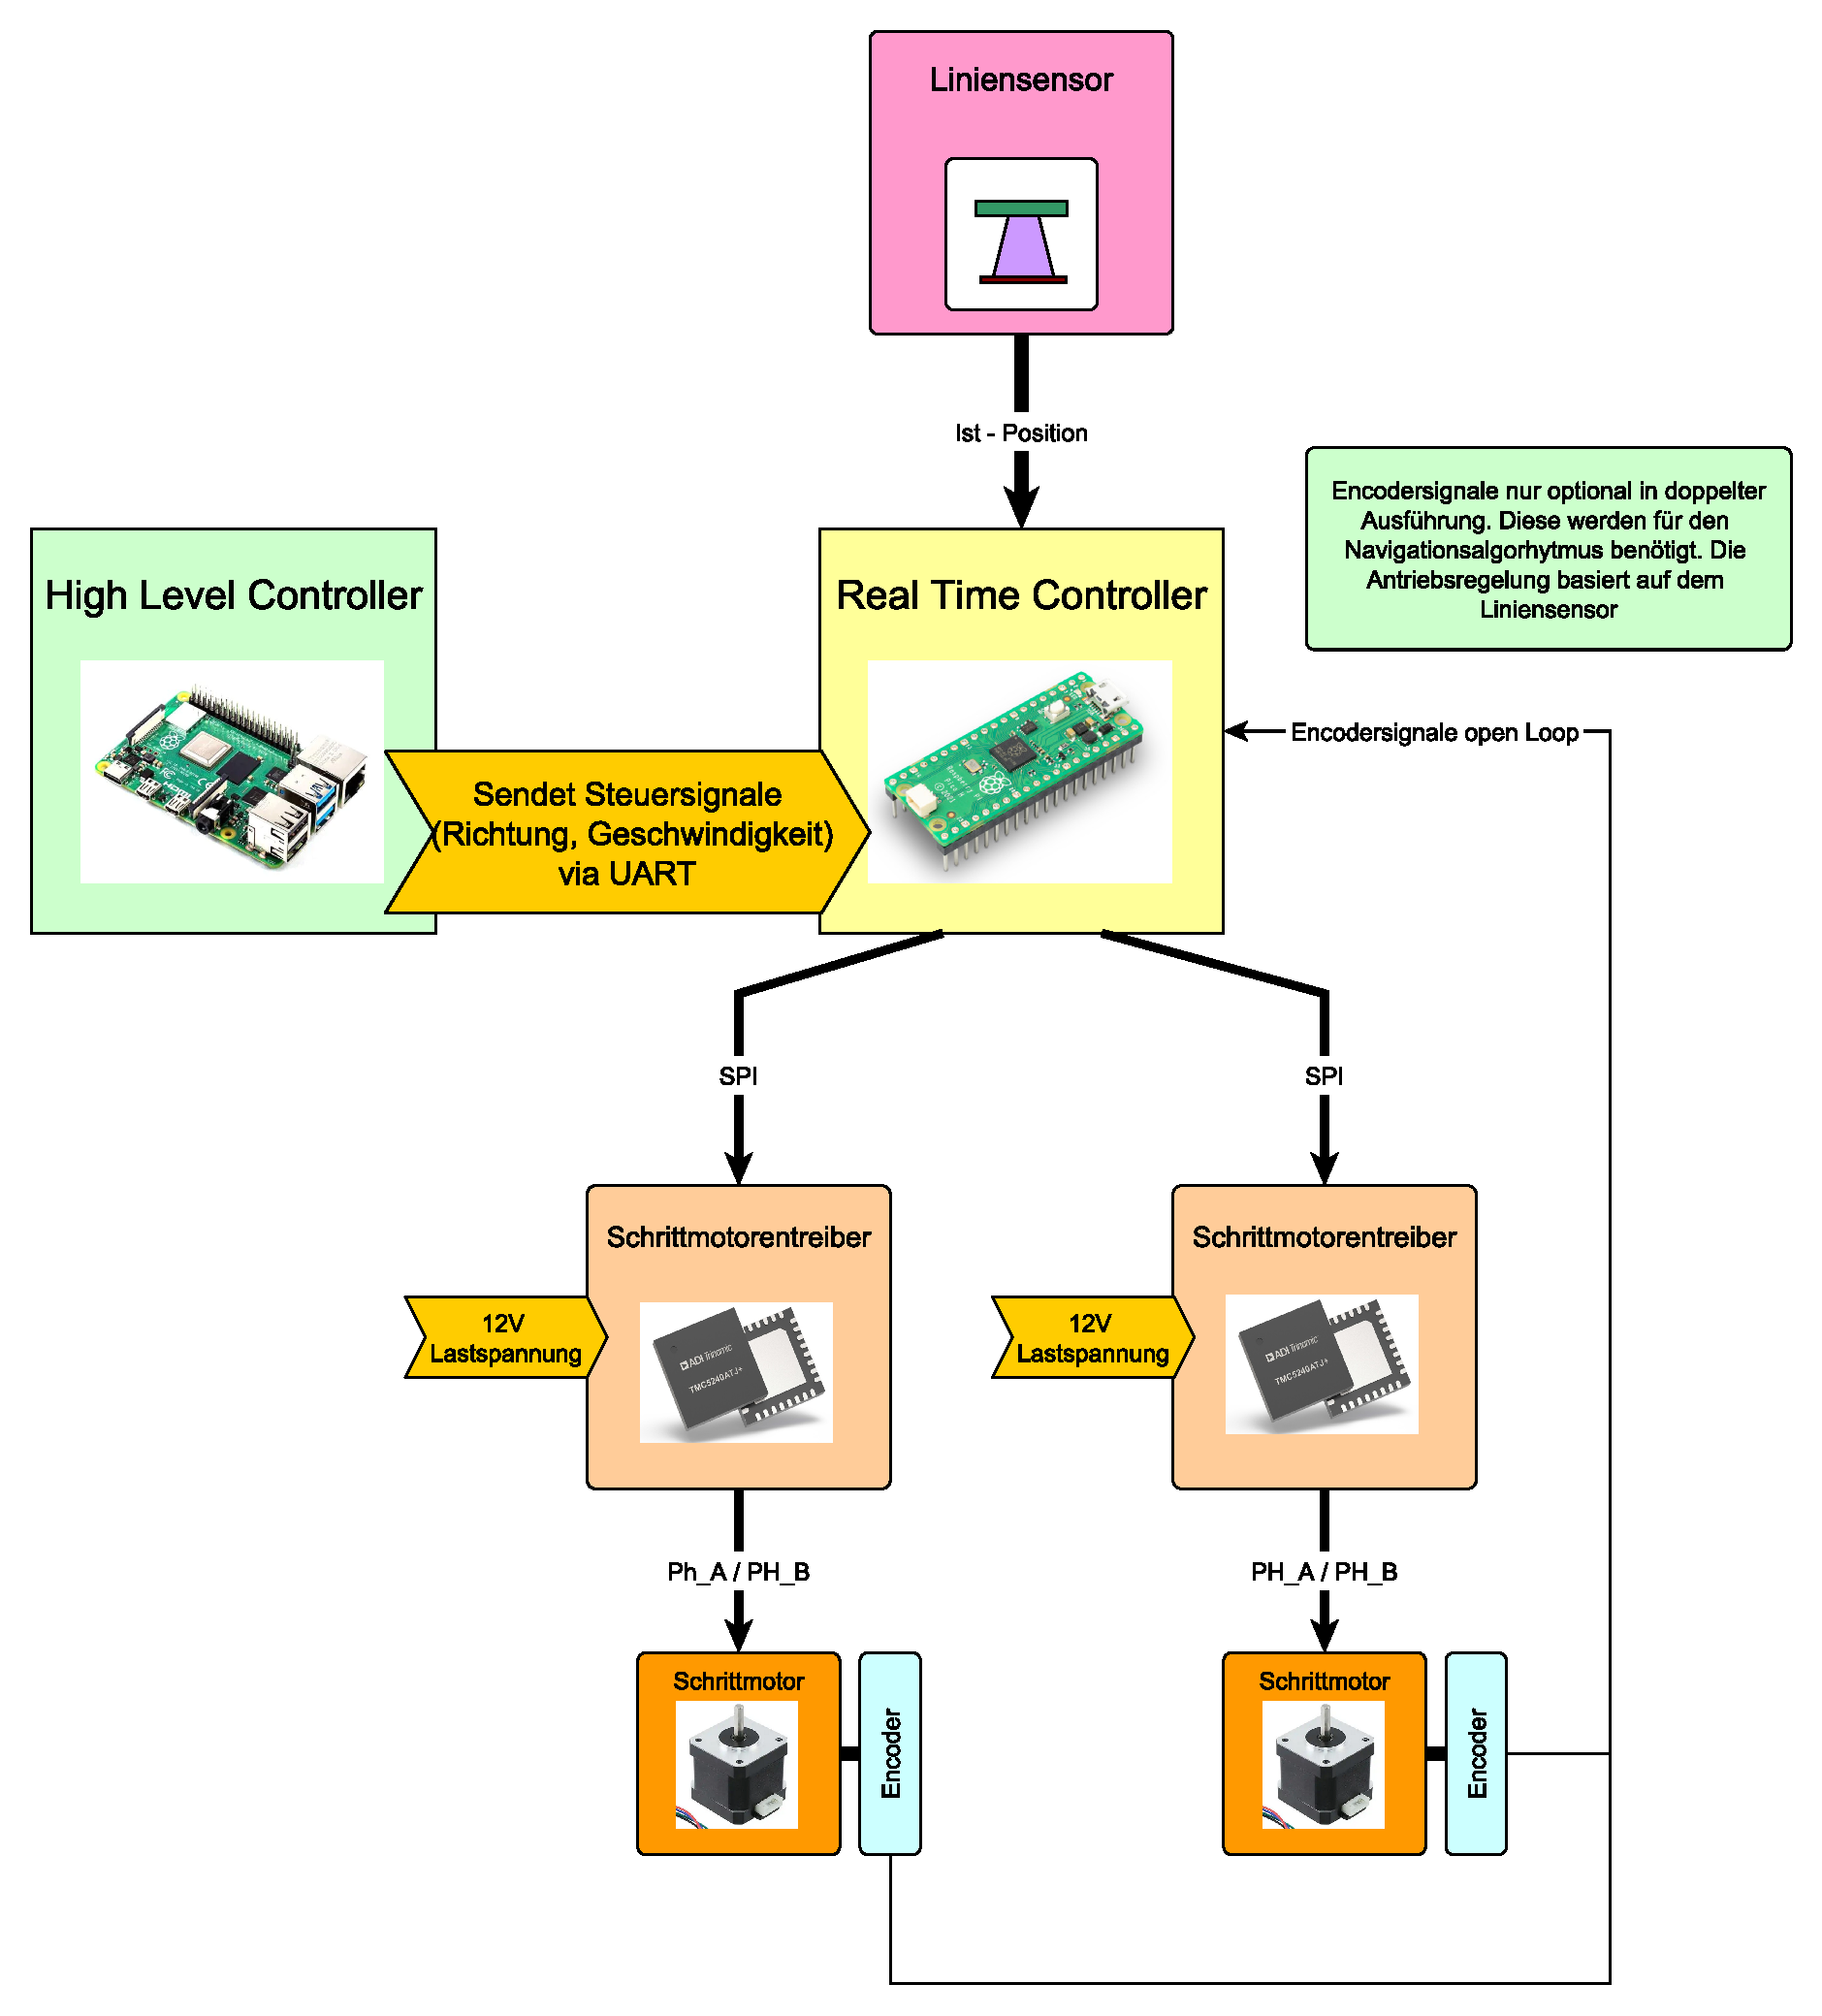
\includegraphics[width = 1\linewidth]{fig_Antriebe_und_Dimensionierung/Konzept_RTC_Trinamic.pdf}
    \caption{Ansteuerungstopologie Schrittmotoren}~\label{Ansteuerungstopologie_Schrittmotorentreiber}
\end{figure}

Die Antriebsregelung wird im Sinne der Gewaltenteilung auf einem eigenen PCB
umgesetzt. Eingangssignale für diesen sind der Liniensensor und 1 oder sogar 2
Encoder. Die Regelung findet allerdings ohne Encoder statt. Die Einganggrösse
dafür ist lediglich die Position des Fahrzeugs auf der Linie. Angesteuert
werden die Schrittmotorentreiber über den SPI-Bus des Microcontrollers.

Die Encoder werden benötigt, damit der Navigationscomputer nachvollziehen kann,
welche Strecke zurückgelegt wurde. Aus Gründen der Echtzeitfähigkeit beim
Auszählen der Encoder werden diese allerdings trotzdem auf der
Antriebssteuerung ausgewertet. Die Encoder sind zum aktuellen Stand des
Projektes eine Fallback-Lösung. Im Nachfolgemodul wird noch evaluiert, ob die
getätigten Schritte, welche aus dem Motorentreiber ausgelesen werden können,
ausreichen können, um die gefahrene Strecke nachvollziehen zu können.

Signale, in welche Richtung das Fahrzeug bewegt werden soll, sowie Start- und
Stopp-Signale erhält der Microcontroller vom Navigationscomputer über eine
UART-Schnittstelle. Der Greifer-Controller kann dem Antriebs-Controller
ebenfalls via UART, Signale übermitteln, welche die Antriebe anhalten - das
Fahrzeug drehen oder eben weiterfahren lassen.

Abbildung \textbf{BILD!!!!!!!!!!!!} zeigt schematisch, welche Funktionsgruppen
das entsprechende Board enthält.

\end{document}
